% Komponentendiagramm des Projektes
\section{Komponentendiagramm}

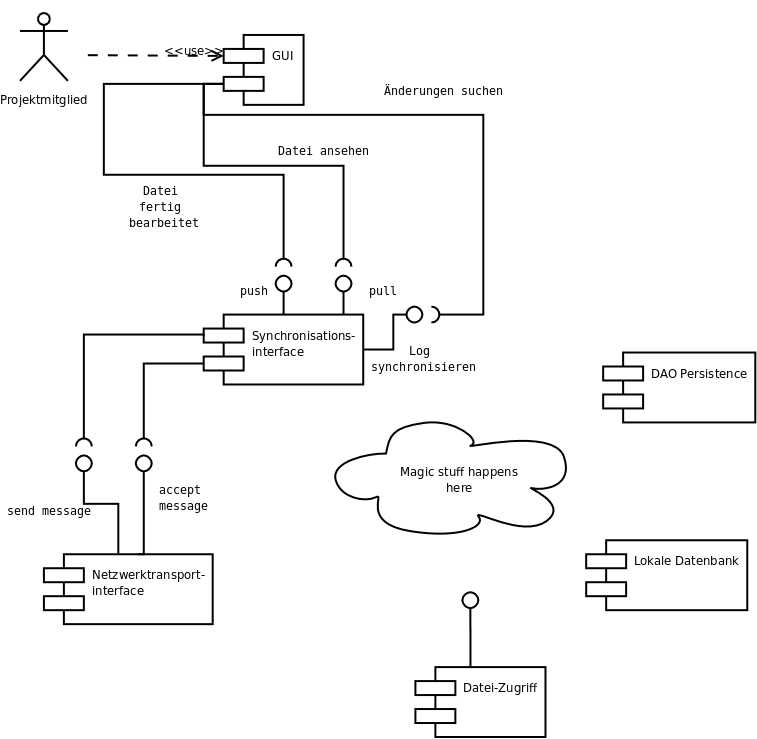
\includegraphics[width=0.98\textwidth]{../uml/component_diagram.png}

Das Projekt ist in folgende 6 Komponenten aufgeteilt:

% Wie man sieht habe ich sehr viel dazugeschrieben. Allgemein ist mein Verständnis von einer Komponente das, dass ich von ihr wissen will, wofür ich sie nutzen kann und was sie mir für Services anbietet. ~simon

% Es sollen zuerst die Aufgaben jeder Komponente beschrieben.
% Danach kann auf Verbindung zu anderen Komponenten eingegangen werden: Nicht durch Abläufe, es sollen die Beziehungen beschrieben werden
% Die Beziehung ist, dass der Core immer die Kontrolle hat, aber dass er eben auch auf Callbacks/Events von den anderen Komponente wartet
% Nicht die internen Abläufe beschreiben, und bei allen Komponenten auf gleichem Detailniveau bleiben. 
% ~johannes


\subsection{Core}
In der Core-Komponente befindet sich die Business Logic der Applikation. Der Core steuert die Funktionalität und die anderen Komponenten, wartet aber auch auf Events/Callbacks von den anderen Komponenten. 
Dies kann etwa das Drücken eines Buttons sein, die Änderung einer Datei im Dateisystem oder eine Nachricht von einem anderen Client. Die jeweilige Komponente wirft einen Event/Callback, den der Core empfängt.

\subsection{Graphical User Interface}
Die grafische Benutzeroberfläche, mit der der Endanwender arbeitet, ermöglicht Zugriff auf alle von der ``Core''-Komponente für Endbenutzer zur Verfügung gestellten
Funktionalitäten.

% Persistence NICHT Database Persistence, es ist nicht festgelegt dass wir eine Datenbank verwenden ~simon
\subsection{Persistence} 
Die Persistence Komponente abstrahiert den Zugriff auf die Daten, die für den Betrieb gespeichert werden müssen. Diese umschließen nicht die Dateien. Es wird das Konzept des Data Hiding umgesetzt, wodurch erreicht werden kann, dass die anderen Komponenten nur auf definierte Weise die Daten verwenden. Für die Speicherung der Daten kann eine relationale Datenbank verwendet werden.

\subsection{Synchronisation Services}
Die Synchronisationskomponente ist für die Verteilung von Änderungsinformationen und Dateninhalten an andere Projektmitglieder/Clients zuständig. 

\subsection{File System Services}
Die File System Services kapselt den Zugriff auf Dateien im Dateisystem. Außerdem kann diese Komponente durch entsprechende Strategien feststellen, ob Dateien geändert wurden oder in die Projektordnerstruktur kopiert wurden und dies dem Core mitteilen, welcher wiederum entsprechende Aktionen veranlasst.

\subsection{Interclient Communication} 
Der Interclient Communication Service kapselt die vollständige Kommunikation zwischen den Clients (über das Netzwerk) und gibt die entsprechenden Nachrichten an den Core weiter. So ist es leicht möglich, verschiedene Netzwerk-backends (z.B. XMPP oder RMI) zu unterstützen, welche für den Core und somit für den Benutzer transparent sind. Außerdem wird die Authentifizierung der Nutzer in dieser Komponente durchgeführt. 
% Ich habe bei Client Authentifizierung ein schlechtes Gefühl. Wenn wir nicht mit XMPP arbeiten, wie werden die Clients dann Authentifiziert? ~simon
% ja. ~johannes